%% Time-stamp: <2023-06-25 18:29:21 vladimir>
%%% Copyright (C) 2019-2023 Vladimir G. Ivanović
%%% Author: Vladimir G. Ivanović <vladimir@acm.org>
%%% ORCID: https://orcid.org/0000-0002-7802-7970

\chapter{Research Design and Methodology}\label{ch:methods}\indent

This dissertation is an \textit{exploratory}, \textit{case study} using a \textit{public policy} lens to examine the \textit{finances} of Rocketship Education. Exploratory means that the precise data that will be collected and the precise methods used to analyze those data are not fully known in advance and will depend on this study's findings as the inquiry evolves. Case studies are in-depth examinations of a single topic that are limited in space or time. Public policy is the set of laws, regulations, rules, and guidelines that affect the actions of an element of society. It is ``the decisions, measures, programs, strategies and courses of action adopted by the government or the legislative body'' \parencite[3]{Knill.Tosun2020}. Public policy mandates, constrains, and abets Rocketship Education's actions and how it structures its finances to meet its goals.

Finance, as it pertains to Rocketship Education, encompasses all transactions of monetary value which involve the legal entities called Rocketship Education (DBA Rocketship Public Schools) and Lauchpad Development, plus other entities with which it has significant financial relationships. An expansive view of Rocketship's finances might also include those of its founders who, perhaps went on to found companies that sold software to Rocketship, and entities focused on real property from whom Rocketship might have bought, leased, or sold real property. The expansive view is beyond the scope of this dissertation.

This chapter contains six sections. The first, \prettyref{sec:process-overview}, describes at a very high level the four steps of inquiry this dissertation will follow. Since understanding how schools are financed is essential to understanding Rocketship's finances, a pair of sections, \prettyref{sec:financing-ca-overview} and \prettyref{sec:charter-school-financing}, will give an overview of school financing in California by describing the normal, common financial disclosures and reports made by all districts and schools and then the essentials of charter school finance. 

% It is important to remember that budgets reflect the future, and audits reflect the past. Budgets are estimates, guesses, projections, whereas audits are a definitive, fixed record of the past. Both are based on assumptions which are usually stated, either in a budget presentation or explicitly noted in an audited financial statement.

The next three sections gone into more depth about charter school finances. The fourth section, \prettyref{sec:real-estate}, covers the varieties of real estate transactions that charter schools might be involved in. The fifth section, \prettyref{sec:gaps-anomalies}, discusses how potential gaps or anomalies in the financial data might be discovered. This is where triangulation can be used to cross-check the validity of that data. % Does everything add up? Are there important, missing documents? How much do these gaps or anomalies matter? Are the oddities long-standing or fleeting? Examples of triangulation might be comparing Rocketship's LCAPs to their budget, or comparing IRS Form 990 data to their audited financial statements.

The last section in this chapter, \prettyref{sec:flows-of-money}, describes how this dissertation will study the flow of money in and out of Rocketship. Until now, this study has treated Rocketship's finances statically, i.e.~at points in time. Just as important are the dynamic flows of money. % Where do they come from, and where do they go?

In order to make what's being analyzed more concrete, \prettyref{appx:ca-school-financing}, contains some example tables drawn from the Los Altos School District (LASD) for the 2019–20 school year. These are standard financial reports taken from LASD's SACS data, but presented in a way that is both visually appealing and informative.\footnote{LASD's annual budgets have consistently won the Meritorious Budget Award for Excellence from the Association of School Business Officials International for the quality and comprehensiveness of its financial statements for each of the last 15 years. Both LASD's annual budget and its CAFR exceed 100 pages. That information and data, although available elsewhere, is truly informative and serves as a record, a history if you will, of LASD's past, its actions, and the data which guided those actions.} The high level view is given in \prettyref{fig:LASD_All_Funds_Summary}. That view is further broken down in five more tables. The final and sixth table is a projection of LASD's of finances for the current year (2018–19), the year whose budget is being presented (2019–20), and five years into the future. The first half of the table contains the assumptions used to generate the amounts in the second half.

The challenge for this inquiry will be to organize the data so that gaps and anomalies can be identified, interesting and valid comparisons can be made with public schools and other charter schools, and the flows of money in and out of Rocketship can be identified. Unlike many studies, there is not a paucity of data on Rocketship, rather there is a surfeit. The data collected so far is voluminous. The current number of pages of initial and renewal petitions runs to 7371 pages for just Rocketship schools in Santa Clara County.\footnote{The massive size of some of these petition calls into question whether authorizers read them in their entirety.} Three bond prospectuses total over 1000 pages. 

\section{Process Overview}\label{sec:process-overview}\indent

Explaining the real estate-related finances of Rocketship Education is the heart of this dissertation. Where do Rocketship's revenues come from? Where are they spending that revenue? Are there investors who make money off of Rocketship? And, critically, if Rocketship takes in more money than it spends on education, where does that money go?

To respond to these questions, the basic process steps for this dissertation will include the following:

\begin{enumerate}
  \item Gather financial data for the Rocketship schools being studied. The initial set of data being analyzed is discussed in \prettyref{sec:charter-school-financing} later in this chapter.
  \item Identify any gaps or anomalies in the data. This is where triangulation is useful and is discussed further in the \prettyref{sec:triangulation}. 
  \item Analyze the flow of money in and out of Rocketship. That  is covered in the section \prettyref{sec:flows-of-money} which tries to determine where Rocketship funds come from, where is that money being spent, and what public policies (or lack thereof) account for Rocketship's actions.
  % \item Identify to the extent possible how people or entities that are not explicitly part of Rocketship Education or Launchpad Development may nonetheless profit from Rocketship's activities. 
\end{enumerate}

Analyzing the finances of Rocketship Education means, for example, determining
the attributes of a particular bond. Are these bonds general obligation or revenue bonds? Are they obligations of Rocketship Education or Launchpad Development and funded their revenues, or are they conduit bonds issued by a government agency and obligations of that government agency that are intended, by not guaranteed, to be funded by Rocketship's revenues? Have the bonds been purchased by entities that are related to Rocketship, i.e.~they are not arm's length transactions? 

All bonds are risky to some extent, some more than others, and purchasers of those bonds are compensated for taking on that risk by being paid interest on the amount borrowed. An immediate question comes to mind: Is the interest rate appropriate for the risk being taken on? Answering that question entails comparing Rocketship Education to other, similar borrowers. If the interest rate is higher than expected, then Rocketship Education is effectively giving away some of its revenue. Another question one might ask is, ``How is Rocketship Education spending its bond proceeds?'' Are those expenses in line with what other charter school chains or public school districts are spending their bond proceeds on? %chktex 38


\section{Financing Schools in California}\label{sec:financing-ca-overview}\indent

Primary and secondary schools (grades TK–12) and charter schools in California are financed with a combination of federal, state, and local monies as seen in \prettyref{fig:2019–20_K–12_Funding}.\footnote{Since federal funds account for only 8\% of total funding for California's elementary school children \parencite{LAO2021}, the federal contribution will not be considered further. Note that federal facilities grants to charter schools are not part of this 8\%.} In June of every year, the California Legislature passes a budget for the next fiscal year (July 1 – June 30) and the Governor signs it into law. This is called the enacted budget and it authorizes the expenditure of funds for programs. This version of the budget describes the \textit{intent} of the Governor and the Legislature, but does not provide any actual money. Funds for programs authorized by the enacted budget are appropriated in \textit{trailer bills} that are passed piecemeal in the months following the adoption of the budget. During the course of the fiscal year, revisions are made to this enacted budget either because of circumstance or because of changed priorities, and at the end of the fiscal year, this is now called the revised budget. After a budget year has passed, technical adjustments are still made: Exactly how much money was spent, or what was misclassified and improperly allocated will change the revised budget numbers. This then becomes the final budget. The upshot of this is that there are actually multiple versions of California's budget: the current year's budget that was passed before July 1\textsuperscript{st}, the previous year's budget, and the budget for the next fiscal year. Normally, when one refers to ``the budget'', which one is dependent on the context.

Budgets in California have a lifecyle. First, the Governor makes a proposal in January, and revises that proposal in May. The Governor and the state legislature negotiate their differences and produce a budget which is passed by the legislature and signed by the Governor. This is the enacted budget.

\begin{figure}
  \centering
  \caption[California 2019–20 K–12 Funding by Source]{\textit{California 2019–20 K–12 Funding by Source}}\label{fig:2019–20_K–12_Funding}
  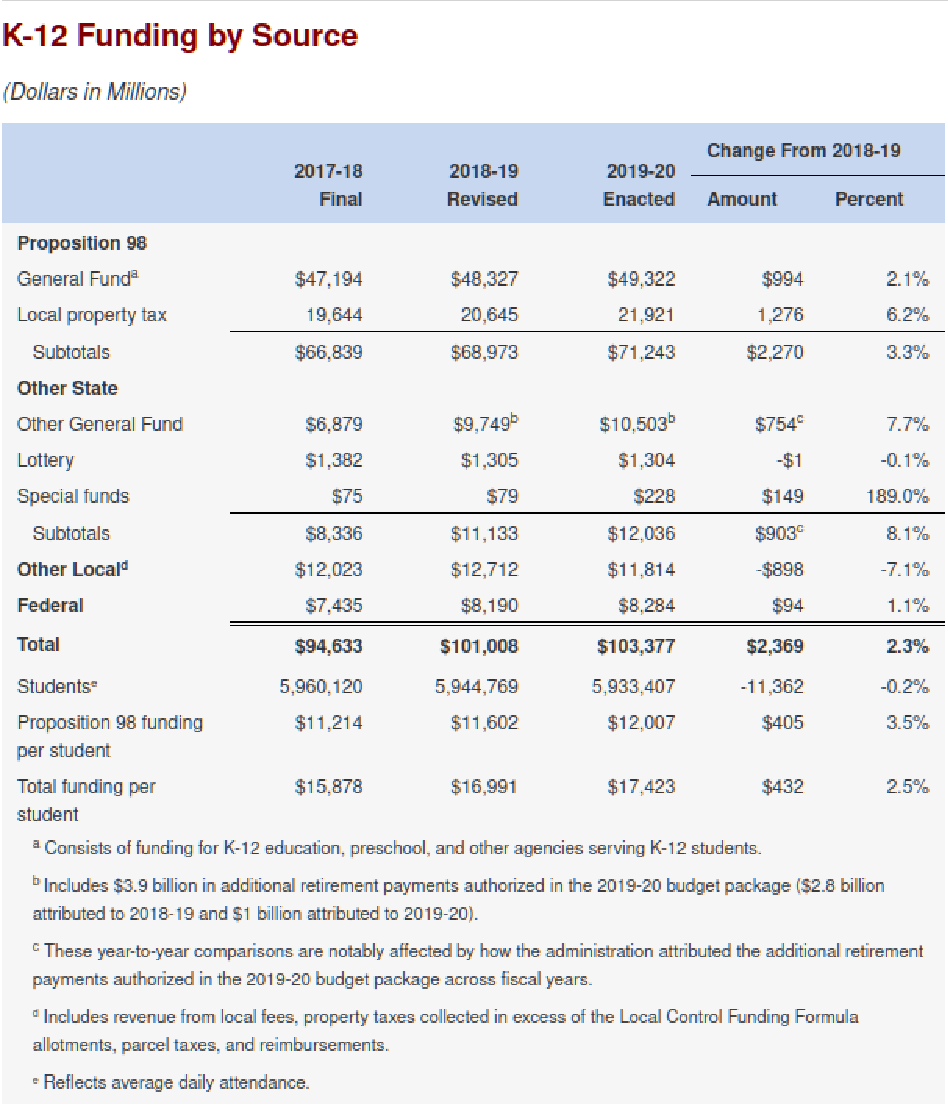
\includegraphics[width=\textwidth]{2019-20_K-12_Funding_by_Source.pdf}\\ %chktex 8
  \footnotesize\raggedright\textcite{LAO2021}.
\end{figure}

\prettyref{fig:2019–20_K–12_Funding} shows what money California has to fund its primary and secondary educational system, i.e.~grades K–12. This money is then allocated to local educational agencies (LEAs), through a formula known as the Local Control Funding Formula (LCFF).\footnote{The LCFF actually funds community colleges as well as public primary and secondary educational institutions, so it ought to be known as funding grades TK-14. Appoximately 89\% of LCFF funding goes to grades TK-12.} LEAs include individual charter schools, county offices of education, and local public school districts. The total amount of money for K–12 funding is allocated using a formula that was enacted by voters in 1988 \parencite{LAO2017}: Proposition 98. Prop. 98 was originally meant to be a minimum guaranteed funding level, but has evolved into a ceiling. The Legislative Analyst's Office (LAO), which serves as an independent, non-partisan research arm of the California Legislature in much the same way that the Congressional Research Service serves the U.S. Congress, calls Prop. 98 ``A Tale of Complexity''  (p.5) and says that ``A Plethora Tests and Rules Govern the Minimum Guarantee'' (p.5), and that ``State Has Made Myriad Adjustments to the Proposition 98 Calculations'' (p.5). Undoubtedly LCFF is complex, but LCFF is more transparent, has fewer rules, is more equitable, and is more responsive to the needs of public school districts that have a high proportion of under-served students than the Revenue Limit System that came before it. The Revenue Limit System was also complex, but in a completely difference way; it had many separately funded programs, called categorical programs, each with their own set of requirements, rules, durations, and funding levels. Each passing year saw more programs being added to the set of categorical programs until the entire collection became bnoth unwieldy and failed to equitably fund K-14 schools.

As seen in \prettyref{fig:2019–20_K–12_Funding}, Proposition 98 funding accounts for nearly 70\% of California's K–12 funding, the remainder coming from local property taxes and fees, and from various other federal and state sources. This money is distributed to county offices of education which then distribute it to public school districts. Districts then distribute funds to charter schools.

Some districts are funded outside of the LCFF system. These used to be called ``basic aid'' districts, but since the term is confusing, they are now called ``community funded'' districts. These are districts whose annual property tax revenue is greater than their annual LCFF entitlement. They get only ``basic aid'', i.e.~the constitutionally required minimum funding (the greater of \$120 per pupil or \$2,400 per district) from the state. For districts which are not community funded, the state contribution is the difference between a district's LCFF entitlement and its share of district property taxes. In other words, the state ensures that each district gets at least its LCFF entitlement, the total amount which is determined by Prop. 98.\footnote{An invaluable and comprehensive description of K-12 funding in California, for both public school districts and charter schools, can be found in \textcite{Aguinaldo.etal2022}, an annual publication.}

\subsection{Budgets \& Interim Reports}\label{sec:budgets}\indent

For a given fiscal year, which runs from July 1\textsuperscript{st} to June 30\textsuperscript{th}, the annual budget is the first of four important financial documents produced. Since budgets must be approved before the start of a fiscal year, they are actually produced and approved in the prior year.\footnote{Since a school's budget must be approved before the state budget is finalized, it is nearly cerain that a school's budget will need to be modified after it has been approved.} The next two financial documents are two (unaudited) interim reports, one in December, and another in March,  which track how well the school or district is adhering to the approved annual budget, and finally, after a certified public accountant has audited the school or district, a comprehensive annual financial report (CAFR) is produced in the fiscal year following the period it covers. State law requires that an independent auditor certify this retrospective account of the school or district's financial activity as being an accurate representation of the school's finances for the previous fiscal year.

\subsection{Local Control Accountability Plans (LCAPs)}\label{sec:lcaps}\indent

An important, recurring, non-financial report of schools is the Local Control Accountability Plan (LCAP). Although the LCAP is a three year plan, it is updated annually. The focus of an LCAP is on the programs that a school (public or charter) is going to implement, finance, and monitor that will allow it meet the goals that the state has set. These are goals that the California Department of Education sets periodically, primarily to ensure that students with the greatest needs are in fact served and are in addition to the seven goals that the Legislature set for charter schools in general.

Typically LCAP goals remain the same over their three year lifespan, but their financing may change if the metrics used to measure progress toward achieving those goals aren't showing progress. In unusual circumstances, how the goals are to be achieved might change. LCAPs are California's way of ensuring that all public schools, including charter schools, meet the same set of priorities or goals. Apparently, some LCAPs have been on the order of 500 pages long, although the norm is much less.

For each activity or group of activities, schools indicate what goal is being met, if the goal includes increased services for disadvantaged student, how well the school or district has met that goal, and how much money has been allocated to achieving and reporting those goals. (The reality of what the Department of Education wants is an order of magnitude more complicated than this description, but it is accurate as far as it goes.)

Unlike budgets and CAFRs, LCAPs don't have to ``add up'', nor do they have to offer a complete financial picture, but they do have to be consistent with other financial data. Expenditures have to be budgeted, and the amounts in a school's budget must agree with what's in the LCAP\@. The charter or public school's board must approve an LCAP at the same time as it approves its annual budget. % chktex 13

\subsection{Comprehensive Annual Financial Reports}\label{sec:CAFRs}\indent

A major source of financial data are the annual, independently audited, comprehensive financial statements of Rocketship Education. Comprehensive Annual Financial Reports (CAFRs) are sent to the California Department of Education (CDE) and to a charter's County Office of Education (COE) annually. They cover the previous fiscal year and are similar to annual budgets because they report the same information, perhaps in a different format. CAFRs are retrospective whereas budgets are prospective. The major difference is that CAFRs are independently audited and budgets are not. 

Similarly to bond underwriters, financial auditors are liable for ``omitting, misstating, or obscuring [items which] could reasonably be expected to influence decisions that the primary users make on the basis of those financial statements'' \parencite{Cayamanda2020}, and this requirement tends to increase the diligence of the auditors. However, potential liability doesn't always result in truly comprehensive financial statements; sometimes the lure of accounting fees overwhelms any misgivings, as was the case with Enron and Arthur Andersen in 2001, and apparently with Donald Trump in 2022. Errors and sloppiness may exist, but in general, fraud is thankfully rare, in part because fraud on the part of auditors would likely result in the loss of the auditor's license, effectively ending their business. 

\section{Charter School Financing}\label{sec:charter-school-financing}\indent

In California, charter schools are financed the same way as public schools are, from the same pot of money, using the same set of rules, except for one significant difference: how they finance facilities. Unlike public schools, charter schools have no taxing authority, so they cannot pass bond measures or parcel taxes. This lack of a taxing authority means that charter schools must either occupy existing public school facilities (potentially displacing existing public school students) or seek grants and donations to fund non-district facilities, either leased or purchased. The federal government provides significant amounts of facilities grant money and delegates to the states the administration of the program and the disbursement of the actual grants. 

An in-depth analysis of charter school finances requires a broader lens than one used for public schools because, in addition to all of the financial dealings of traditional public schools, almost all of which also apply to charter schools, charter schools have large and immediate needs for facilities that traditional public schools don’t have. This brings into the picture bonds, loans, grants, leases, construction, and the purchase and sale of real estate. Traditional public schools do issue several kinds of bonds, levy parcel taxes, and buy real estate on which they build schools, but they do so infrequently.Usually public schools have done this years ago, but charter schools have an immediately and reoccurring need for facilities. They face these needs once when they start up, and whenever they outgrow their facilities because of increased enrollment. These needs of charter schools for facilities and the financing associated with obtaining those facilities is more pressing, more immediate, and more common than the corresponding needs of traditional public schools whose enrollment doesn't fluctuate as much.\footnote{Usually a public school district sees a change in enrollment because of significant demographic changes like immigration or emigration, birth rate increases or declines. Charter schools can see enrollment changes absent any demographic change, even if the total number of students residing in a district stays the same. In some instances, increased enrollment in charter schools comes from public school students switching from the public school system to charter schools. This is what is happening to Oakland, CA and it produces simultaneous but opposite changes in enrollment.}

\subsection{Charter Financial Documents}\label{sec:charter-financial-docs}\indent

Only a few financial statements are needed to get a good overall picture of a school's or district's finances. These are the enacted annual budget and interim reports, the audited Comprehensive Annual Financial Report (CAFR), parts of the Local Control Accountability Plan (LCAP), and for charter schools, the financial portions of their petitions.

Fortunately, there are numerous publicly available sources of charter school financial data. The entire set of publicly available financial data from charter schools are, in roughly chronological order, petitions/renewals, budgets, LCAPs,  interim financial statements, and finally, audited Comprehensive Annual Reports (CAFRs). \prettyref{tab:charter-fin-docs}, summarizes the official, publicly available, and required financial reports about charter school finances. Note that budgets, interim reports, LCAPs, and CAFRs are also required of public schools.

There is one source of financial data that is not official

\begin{table}[h]
  \centering\small%
  \caption[Charter School Financial Documents]{\textit{Charter School Financial Documents}}\label{tab:charter-fin-docs}%
  \begin{tabular}{llll}
    \toprule%
    \multicolumn{1}{c}{Name}  & \multicolumn{1}{c}{Description} & \multicolumn{1}{c}{Frequency} & \multicolumn{1}{c}{When} \\
    \midrule%
    Initial Petition  & Comprehensive description    & Once           & Before opening \\
    Renewal Petitions &  Similar to initial petition & Every 5 years  & Years 5, 10, 15, \ldots \\
    Budget            & Complete financial plan      & Annually       & Before June 15\textsuperscript{th} \\
    LCAP              & How to meet state priorities & Every 3 years  & With budget\\
    Interim Reports   & Current spending             & Twice yearly   & December, March \\
    CAFR              & Audited financials           & Annually       & In the following year \\
    \bottomrule%
  \end{tabular}
\end{table}%

\subsubsection{Petitions \& Renewals}\label{sec:petitions-renewals}\indent

Viewed chronologically, the first financial statement from a charter school is contained in their initial petition. Before a charter school is allowed to begin operation, every charter school in California is required to present to a chartering authority a petition which must contain certain required elements. The absence of one of these elements is grounds for denying the charter's petition to operate. For example, what is the intent of the charter school? How is the charter school going to measure its success or failure? What population is it targeting? And, what are its financial projections?

A financial projection is one of the required elements of any petition is a financial projection. Although no one expects a charter school (or any public school district for that matter) to prepare and adhere to a budget that exactly matches what's been projected, budgets are expected to be a reasonable approximation of future revenues and expenses.

Petitions run anywhere from a hundred or so pages to over a thousand. They contain a wealth of data on curriculum, demographics, pedagogy, discipline, teacher recruitment, and, of course, on the charter school's finances. Fortunately, these documents are all publicly available and could, if needed, be the subject of a California Public Records Act (CPRA) request. The CPRA is the California equivalent of the federal Freedom of Information Act (FOIA). Many of the documents mentioned in this dissertation are available from the California Departments of Education and Finance, or from the Santa Clara County Office of Education.\footnote{Since these documents are publicly available and may be freely copied, so no copyright is applicable, nor can one be claimed.}

Since Rocketship schools are all operated by a single entity, (currently) Rocketship Education, DBA Rocketship Public Schools, a 501(c)(3) non-profit, their financial statements and those of their affiliates are rolled up into a single document, the Consolidated Financial Statements and Supplementary Information. Every school is included in this single document, as are separate Launchpad Development LLC's that own facilities leased to individual schools. % chktex 36

\subsubsection{Budgets}\label{sec:budgets}\indent

Once a charter has been granted the right to operate, it must file annually with the California Department of Education, just like public school districts, certain forms that detail its revenues and expenses. State law also mandates an annual audit by an independent accounting firm which charter schools must file with their County Office of Education. All together, these forms should provide a complete picture of a charter school's finances, and crucially, everything should be in agreement. Charters must approve and publish at a public meeting their annual budget, and they, just like traditional public schools, cannot spend unbudgeted money unless the governing board approves any changes at a public meeting.

\subsubsection{LCAPs, Interim Reports, and CAFRs}
\label{sec:lcaps-interim-reports}\indent




\subsection{Other Data}\label{sec:other-data}\indent

Vast amounts of data are available from the federal, state and  local governments, easily over half a million datasets each containing anywhere from a hundred elements to a hundred thousand elements. Unfortunately these data have been collected in different formats, over different time periods, using different inclusion criteria, more or less carefully. Picking a subset of educational data to use and then cleaning it is a huge endeavor well beyond the scope of this dissertation. That being said, a very small subset of available datasets will be consulted, based on the immediate need at hand. The most likely datasets to be consulted are those maintained by:

\begin{itemize}
  \item California Department of Education and the State Board of Education
  \item The County of Santa Clara and the Santa Clara County Office of Education
  \item The California Open Data Portal
  \item National Center for Education Statistics (NCES) at the Institute for Education Sciences (IES)
  \item Stanford Educational Data Archive (SEDA)
  \item School Finance Indicators Database
  \item EdSource, Ed-Data, and other aggregators of educational data specific to California
\end{itemize}

\subsubsection{State and Federal Filings}\label{sec:state-federal-filings}\indent

Two filings are of particular interest: FPPC Form 700, Statement of Economic Interests, and IRS Form 990, Return of Organization Exempt from Income Tax. Both forms force the disclosure of personal financial information (Form 700) or personal financial information and business financial information (Form 990). 

Some officers of Rocketship may be required to submit annually to the California Fair Political Practices Commission (FPPC) Form 700, Statement of Economic Interests. This particular requirement of charter school officers is not settled law, but if Form 700 is filed, it will list the submitter's assets and income that are related to the position they hold in Rocketship Education or Launchpad Development. The intent is to prevent related-party transactions by enumerating an officer's economic interests so that a school can avoid doing business with entities that might benefit an officer. Rocketship's initial petition for Mateo Sheedy states that Form 700, Statement of Economic Interest, shall be filed by all board members, candidates for board membership, corporate officers, principals and assistant principals, among others. 

The federal Internal Revenue Service grants income tax exemptions to organizations that meets the requirements of §501(c)(3) of the  Internal Revenue Code.\footnote{26 USC 501, i.e. Title 26, Subtitle A, Chapter 1, Subchapter F Part I § 501(c)(3)} These organizations must file Form 990 annually that provides some minimal financial data. (Tax returns of for-profit organizations are not public documents and their contents do not have to be disclosed; however, in order to sell stock to the public, i.e.~to be listed on a stock exchange, firms are required to publish various financial documents, which like bond prospectuses, are required to be informative and complete.) %chktex 36

\subsubsection{Bond prospectuses}\indent

Bond prospectuses are also a source of financial information. When bonds are issued, their terms (e.g. interest rate, repayment schedule, collateral, etc.) are described in great detail in a prospectus. These prospectuses, in addition to specifying the terms of the bond, contain information, again in great detail, relevant to assessing the risk associated with purchasing that bond. Bonds are loans, and when millions of dollars are being loaned, those making the loans want to be assured of getting paid back and paid back on time.

Bond prospectuses can be mined for data that might not appear in petitions or financial statements because bond underwriters are ``potential liability for any material misrepresentations or omissions contained in a registration statement or prospectus'' \parencite{Block.etal2008}. This liability, of course, is not unlimited. If bond underwriters exercise due diligence or the misrepresentation is not material, the underwriters are probably not liable. Crucially, the definitions of \textit{material misrepresentation} and \textit{due diligence} depended on both statute and case law, so a bond underwriter can only make a reasoned guess at their exposure to liability. The result is that bond underwriters are likely to be more diligent that is absolutely necessary.

\section{Charter Schools and Real Estate}\label{sec:real-estate}\indent

Charter schools in California must obtain the facilities they plan to occupy before they receive any per-pupil state funding.Unlike many studies, there is not a paucity of data on Rocketship, rather there is a surfeit. The data collected so far is voluminous. The current number of pages of initial and renewal petitions runs to 7371 pages for just Rocketship schools in Santa Clara County.\footnote{The massive size of some of these petition calls into question whether authorizers read them in their entirety.} Three bond prospectuses total over 1000 pages. 

The challenge for this inquiry will be to organize the data so that gaps and anomalies can be identified, interesting and valid comparisons can be made with public schools and other charter schools, and the flows of money in and out of Rocketship can be identified. One approach would be to create a common framework and recast all the financial data from each school into that common framework. But, until the data have actually been collected and analyses started, choosing one particular framework within which to work is likely to lead to work which will need to be redone using a different framework.

 As shown in \prettyref{tab:charter-facilities-options}, they have three options: co-locate, lease, or buy.

\begin{table}[ht]
  \small%
  \caption[Charter School Facilities Options]{\textit{Charter School Facilities Options}}\label{tab:charter-facilities-options}%
  \begin{tabular}{ll}
    \toprule%
    Option    & Description \\
    \midrule%
    Co-locate & \multirow[t]{2}{4.75in}{The charter school occupies ``reasonably equivalent'' facilities provided by 
    the public school district in which the charter school is located.}\\\\
    Lease     & The charter school occupies facilities that it leases.\\
    Own       & The charter school buys existing facilities or builds their own. \\
    \bottomrule%
  \end{tabular}
\end{table}

\subsection{Co-Locating}
\label{sec:co-locating}\indent

The least costly option for charter schools is to co-locate in an existing school. Proposition 39 and enabling regulations\footnote{Ed. Code §47614 et seq. and 5 CCR § 11969.1} require that school districts furnish facilities for all in-district charter school student that are reasonably equivalent to those of students in the district in which the charter school resides. Facilities include regular and specialized classrooms, administrative offices, playgrounds, and athletic fields. It doesn't matter if the school district has unused space or not. It doesn't matter if the charter school grows in enrollment year over year. School districts are required to furnish reasonably equivalent facilities under Proposition 39. However, districts and charter schools may enter agreements outside of Proposition 39 concerning what facilities districts will provide to the charter school.

In theory co-locating is the least costly and most timely option for charter schools to obtain facilities, but often there is litigation over the extent or appropriateness of the facilities that the district has provided. Sometimes these lawsuits can drag on for years, often at a considerable expense for both the charter school and the public school district supplying the facilities.

\subsection{Leasing}\label{sec:leasing}\indent

Charter schools may lease their facilities from either a related party, or at arms length, from an unrelated party. Terms and length of leases vary. If the lessor is an unrelated party, the charter schools may take advantage of grants offered by the Charter School Finance Authority authorized by California SB740\footnote{Ed. Code §47614.5 et seq. and CCR §10170 } ``to offset annual on-going facility costs for charter schools that service a high-percentage of students eligible for free or reduced-price meals (FRPM) or located in a public elementary school boundary serving a similar demographic'' \parencite{CATreasurer2023}. The amount of the grant is the lesser of the school's ADA × \$1,420 or the annual rent × 75\%\footnote{This is the basic calculation. As expected, there are variations and permutations, and these are enumerated in Section 6, Grant Award Calculations of the program's FAQ\@. The principle limitation is that the charter school must serve.} To be eligible, charter schools must ``service a high-percentage of students eligible for free or reduced-price meals (FRPM) or [be] located in a public elementary school boundary serving a similar demographic'' \parencite{CATreasurer2023}.

If the charter school is leasing from a related party, usually SB740 grants are not available. However, the definition of \emph{related party} does not include non-profit entities whose only business is supporting charter schools. For example, a non-profit charter school may lease a property from a related non-profit entity whose only business is owning and maintaining that property. This is the relationship that Rocketship Education has with the owners of the facilities they lease. The structure of Rocketship Education is diagrammed in \prettyref{figp:RSED-corporate-structure}.

\subsection{Owning}\label{sec:owning}\indent

The third way of obtaining facilities is to own the needed facilities, or to have a related party own the facilities. These might be purchased, or the land purchased and the facilities constructed. Most public school districts own their own facilities, but since these were likely bought and built using bond money derived from taxes, charter schools, lacking taxing authority, are unable to pay for their facilities this way.

Instead, charter schools have a few options, shown in

\begin{table}[ht]
  \small\OnehalfSpacing%
  \caption[Options for Paying for Facilities]{\textit{Options for Paying for Facilities}}\label{tab:paying-for-facilities}%
  \begin{tabular}{ll}
    \toprule%
    Option    & Description \\
    \midrule%
``    \protect\smallskip%
    Private grants & \multirow[t]{2}{4.75in}{The charter school uses a grant from an individual, a venture fund, or a foundation to pay for facilities.}\\\\
    \protect\smallskip%
    Federal or State grants & \multirow[t]{2}{4.75in}{Both the Federal government and states have programs which offer funds that may be used to pay for existing facilities or for new construction.}\\\\
    \protect\smallskip%
    Tax credits & \multirow[t]{2}{4.75in}{The federal government offers tax credit for investors whose investments meet certain criteria.}\\\\
    Bonds & \multirow[t]{2}{4.75in}{Charter schools may use the commercial or municipal bond markets to obtain funds, but property or parcel taxes may not be used to pay them off.}\\\\
    \bottomrule%
  \end{tabular}
\end{table}

\subsubsection{Tax Credits}\label{sec:tax-credits}\indent

Tax credits are often used as a source of funds to buy or construct facilities. For example, the New Markets Tax Credit is a 39\% tax credit, usable over seven years, available to those who make an investment in specified economically depressed neighborhoods. A 39\% tax credit is roughly twice the current corporate tax rate which means that this credit wipes out the taxes on gains equal to twice the initial investment (which may itself also have a return). 

\subsubsection{Venture Funds}\label{sec:venture-funds}\indent

The NewSchools Venture Funds, the Charter School Fund, and the Charter School Growth Fund are just a few examples of venture funds that specialize in charter schools. Since it is unlikely that investors will invest in a fund that does not return a profit, establishing exactly how these funds turn a profit is going to be a goal of this study's explorations.\footnote{It is interesting that none of the web sites of these funds mentions that fund's return on investment (ROI). The absence of any indication of a return on investment is either an innocent mistake or much more likely, an attempt at obfuscation.}

\section{Are There Gaps or Anomalies in the Data?}\label{sec:gaps-anomalies}\indent

All of the sources of data mentioned above should be in basic agreement, i.e.~the LCFF funding received by a Rocketship charter school should match what the state thinks it's sending to the school, what the school reports to the state it received and spent, what independent auditors report the school received and spent, and what it actually spent. Further, bond prospectuses and Security Exchange Commission (SEC) filings should be in agreement and with sbudgets. If these figures are not in agreement, something is amiss and should be investigated.

In some fashion or another, all profit must originate from Rocketship's revenue. In the case of the sale-leaseback of facilities, for example, the rent over and above market rates constitutes profit to the property owners, and this is an operational expense ultimately paid for by tax payers. If facilities are bought with public dollars (i.e.~federal grants) and subsequently sold, the net proceeds are profit that might accrue to an organization other than Rocketship. If technology is being used and the contracts are not at arm's length, then someone or some organization is making more than the usual profit. If student data is being sold by a for-profit entity that operates non-profit charter schools, that's revenue that rightfully belongs to the students or to the non-profit schools. 

Determining whether there are gaps or anomalies in a charter school's financial data is time-consuming but not very complex. When examining financial statements, one should be alert to unusual year-to-year changes, ratios (e.g. salaries to total expenses) that are markedly different from the norm, entries that are missing components, or entries that are not supported by detail elsewhere. Complex third-party transactions that don't seem to add value are also indicators that further investigation is needed.

In the search of gaps or anomalies, one might ask questions such as:
\begin{itemize}
\item Are the data available and accessible? Charter schools are notorious for simply not filing required documents or filing them horrendously late, or submitting documents that are incomplete. Petitions are not usually a problem because without a petition, or with a materially incomplete petition, the petition will not be granted. However, once a school is operational, late or missing filings will not bring everything to a halt. Although Rocketship was fined for failing an attendance audit, it was allowed to continue to operate.
  \item Have the data been misrepresented? There are forensic techniques (e.g. Benford's Law) that can point to suspect data \parencite{Zhu.etal2021}. There is also triangulation which involves comparing one source of data with another to see if they match. For example, charter petitions make forecasts of revenue and expenses. How accurate were those forecasts? Were the reasons given for anomalies plausible? foreseeable? reasonable? Following Hanlon's Razor\footnote{``Never attribute to malice that which is adequately explained by stupidity.'' Naturally, Hanlon's Razor follows Stigler's Law of Eponymy: ``No scientific discovery is named after its original discoverer.'' Stigler's Law adheres to Stigler's Law.}, a single anomaly is not usually a sign that something is being covered up, but several persistent anomalies usually are. %chktex 12 38
  \item California requires that LEAs meet the numbers they previously forecast or explain why they didn't meet those numbers. Were those goals met, and if not, were the reasons proffered legitimate? When preparing a budget, LEAs must also certify they can meet their financial obligations for the current year, and for the next two years. If an LEA cannot certify that they can, they might receive a visit from the California Department of Education's Financial Crisis \& Management Assistance Team (FCMAT), and in the extreme case be subject to a state takeover or to involuntary closure. 
\end{itemize}%

\subsection{Triangulation}\label{sec:triangulation}\indent

Another technique for determining if there are gaps or anomalies is to use triangulation. Triangulation is the use of multiple sources of data. While triangulation in social science research often refers to the mixed methods use of quantitative and qualitative methodologies, the common definition refers to the analysis of multiple forms of corroborating evidence in the form of financial and media documentation. For example,  \textcite{Bhandari2022} notes that one of the forms of triangulation is ``[u]sing data from different times, spaces and people'' and also that ``[t]riangulation in research means using multiple datasets, methods, theories and/or investigators to address a research question. It’s a research strategy that can help you enhance the validity and credibility of your findings.''\footnote{Triangulation does not imply exactly three concepts or ideas; often, as is in this dissertation, more than three concepts, ideas, data are combined in the analysis.}


\section{Are There More Serious Financial Issues?}\label{serious-problems}\indent

Unfortunately, charter schools and charter school chains have a long history of various kinds of fraud. \textcite{Lafer2017}, \textcite{ITPT2018}, \textcite{Burris.etal2020}, and \textcite{Burris.Bryant2020}, are just a few of the reports that detail fraud and waste in charter schools. Although Rocketship has engaged in a number of questionable activities, it has not been charged anything illegal.\footnote{Rocketship schools in Santa Clara have had ties with a virtual charter school serving special education students hundred of miles away. They have collected pandemic-relief funds intended for businesses and not available to public schools. Rocketship has been the subject of several Letters of Concern from the California Department of Education, and it has had petitions to open schools denied for substantive reasons. Many of these issues have been collected and can be viewed at \url{https://www.scoop.it/topic/charter-choice-closer-look} \parencite{Marachi2022}.} But with billions of dollars allocated to charter schools for facilities in the last 15 years in California alone \parencite[4]{Lafer2017}, coupled with lax or no oversight, the temptation to misappropriate funds must be strong. It is also instructive to note that Californian charter schools have fought tooth and nail to prevent any laws that would increase transparency or hold charter operators to the same conflict-of-interest standards that public schools and other government entities are held to. While the charter sector has for the most part been successful in warding off demands for accountability, the Attorney General of California issued an official ruling in 2018 stating that the Brown Act, the CPRA, and Government Code §1090 apply to charter schools as well as to other LEAs \parencite{Becerra.Medeiros2018}.

However, it's not necessary to misappropriate funds to make money off of charter school facilities. As the report \citetitle{ITPT2018} from \citeauthor{ITPT2018} details,

\begin{quotation}\noindent\OnehalfSpacing%
While charter schools constructed with general obligation bonds cannot be sold or used for anything other than the authorized school, schools constructed with tax-exempt conduit bonds become the private property of the charter operator. Even if the charter is revoked, neither the state nor a local school district can take control of this property. Additionally, schools constructed with private funding subsidized by New Market Tax Credits or acquired with private funds but whose mortgage payments are reimbursed through the Charter Facilities Grant Program (known as “SB740”) are typically owned without restriction.\\ \sourceatright{\parencite[6]{ITPT2018}}
\end{quotation}

Rocketship has issued just shy of \$90M of tax-exempt bonds to ``finance and/or refinance the acquisition, construction,
expansion, remodeling, renovation, improvement, furnishing and equipping of the land and facilities''  \parencite{CSFA2015,CSFA2015a,CSFA2016,CSFA2017,CSFA2017a}. These conduit bonds are exactly the kind referenced in \textcite{ITPT2018}. The properties owned or leased are (partially) paid with public funds but are privately owned.

\subsection{Analyzing Rocketship's Bond Financing}\indent

Bond financing can be both complicated (a hard problem, but solution methods exist) and complex (many unknowns and interrelated factors). Illustrating this are two examples of the analysis from just a single prospectus, that of Rocketship's \$42M bond offering. That offering is described in the 536 pages which comprise \citetitle{CSFA2017a}. The \$42M offering is complicated because there are many moving parts which are described in the offering in the well-known language of bond finance. Terms, rates, contingencies, amounts, dates, and required performance are all specified in a fashion that has withstood legal onslaught many times over. But the offering is also complex because it must also convince others that its predictions are reasonable. The most important of those predictions is that the issuer can pay the interest and repay the principal when they due.

\prettyref{fig:flow_of_funds_overview} gives the overall picture and shows how rents from schools (blue) are ``intercepted'' by the California Controller (red) and paid directly to landlords, or paid into the Gross Revenue Fund (red) from which the Master Trustee pays lessors (orange) and bond holders and expense accounts (orange). What is not shown is the \$750 per ADA (in 2017, rising to \$1,211 in 2020–21) that Rocketship will apply to lease payments. Since money is fungible, the State of California is giving Rocketship between \$2.4 and \$3.7M depending on the year, money they would otherwise not have. This is effectively profit.

\begin{figure}[hbt]
  \centering
  \caption[Flow of Funds: Overview]{\textit{Flow of Funds: Overview}}\label{fig:flow_of_funds_overview}
  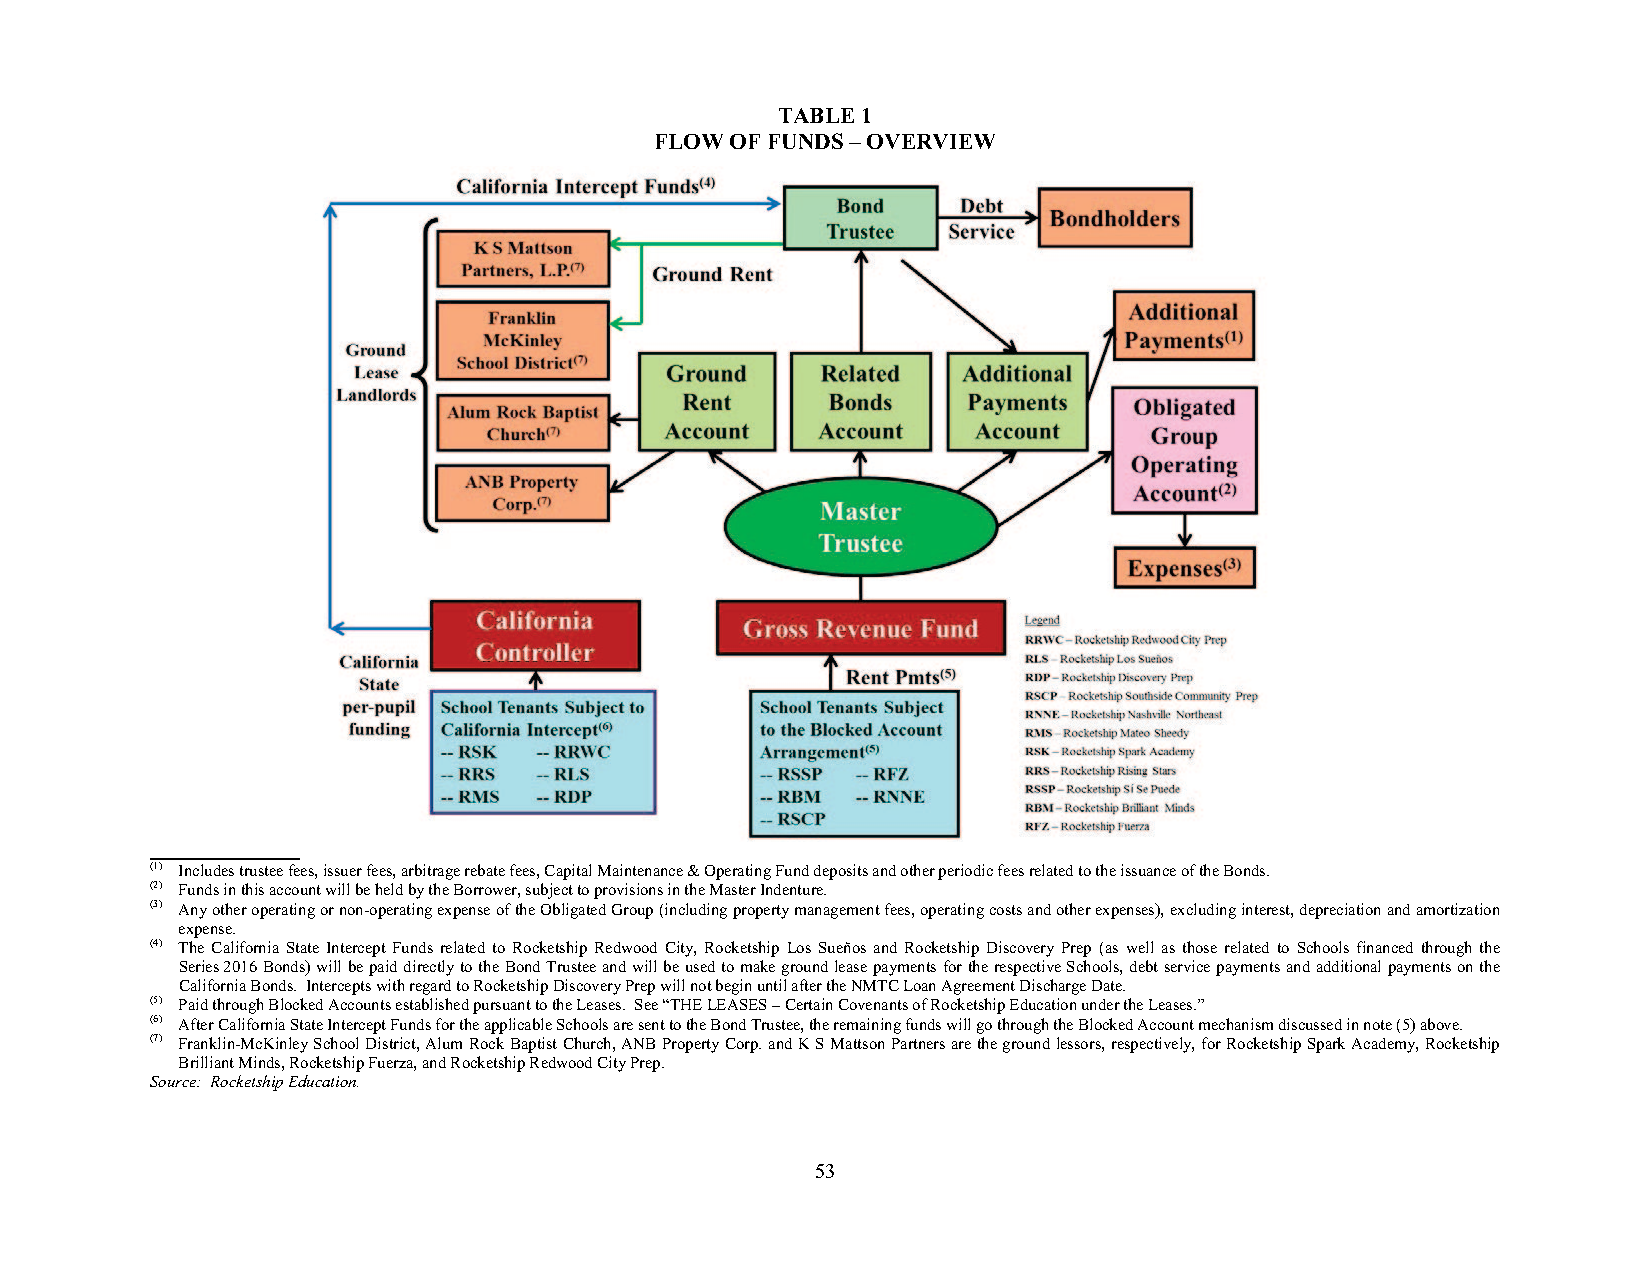
\includegraphics[width=\textwidth]{Flow_of_Funds_Overview}\\
  \footnotesize\raggedright\textcite[53]{CSFA2017}. 
\end{figure}

The next figure, \prettyref{fig:flow_of_funds_cross-collateralization} adds an important detail: how Rocketship uses its assets as collateral more than once.\footnote{\textit{Cross-collateralization} means using an asset as collateral for two or more obligations, here lease and bond payments.} In this case, if the payments of ``School Tenants'' are insufficient, the Master Trustee may require additional monthly payments from the ``Obligated Group Representatives and Member'' to supplement those from ``School Tenants''. 

\begin{figure}[hbt]
  \centering
  \caption[Flow of Funds: Cross-Collateralization]{\textit{Flow of Funds: Cross-Collateralization}}\label{fig:flow_of_funds_cross-collateralization}
  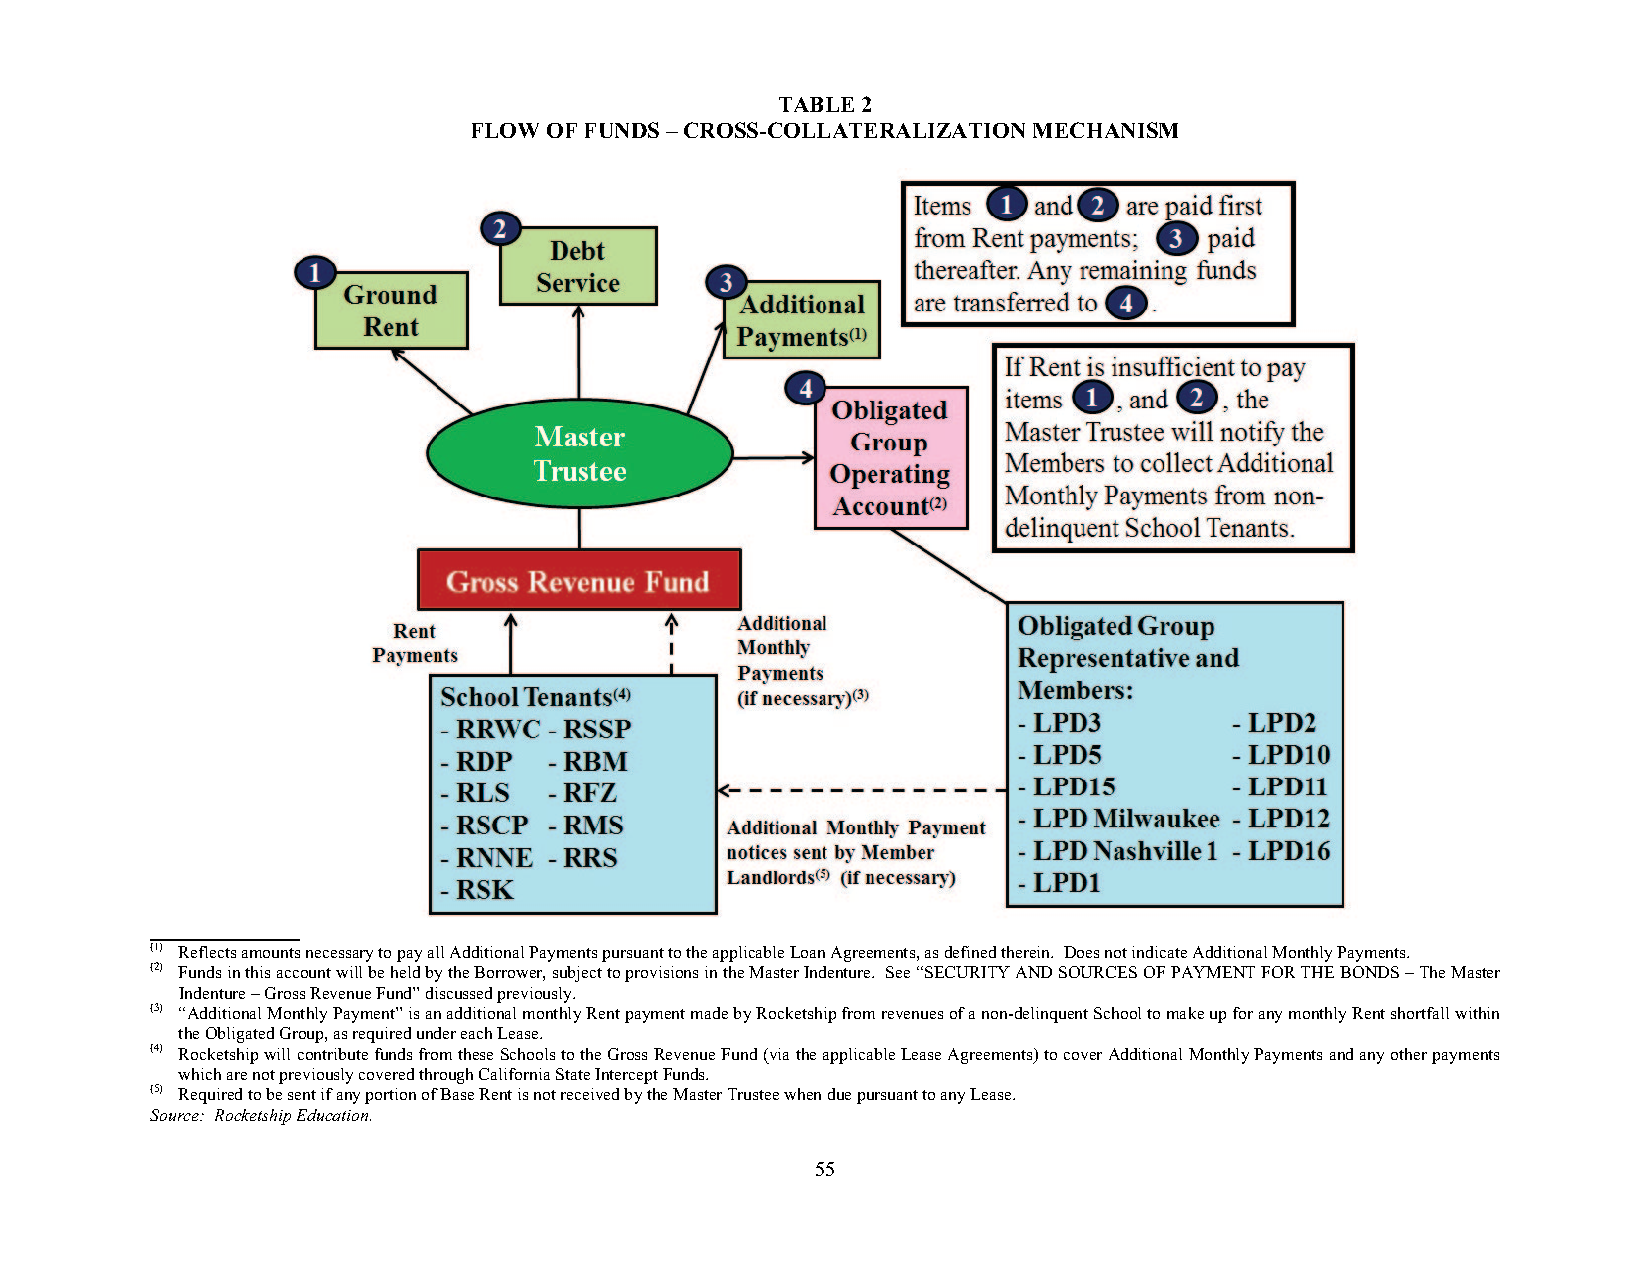
\includegraphics[width=\textwidth]{Flow_of_Funds_Cross-Collateralization}\\
  \footnotesize\raggedright\textcite[55]{CSFA2017}.
\end{figure}

These two examples show the kind of analysis that is needed to characterize a bond offering.


\section{The Flow of Money Through Rocketship?}\label{sec:flows-of-money}\indent

Since a goal of this dissertation is to map the flow of money into and out of Rocketship, I will use diagrams similar to the one used by \citeauthor{Baker.Miron2015} (\citeyear{Baker.Miron2015}), which is reproduced here as Figure~\ref{fig:opresflows}.
\begin{figure}[ht]
  \centering
  \caption[Operating Resource Flows]{\textit{Operating Resource Flows}}\label{fig:opresflows}
  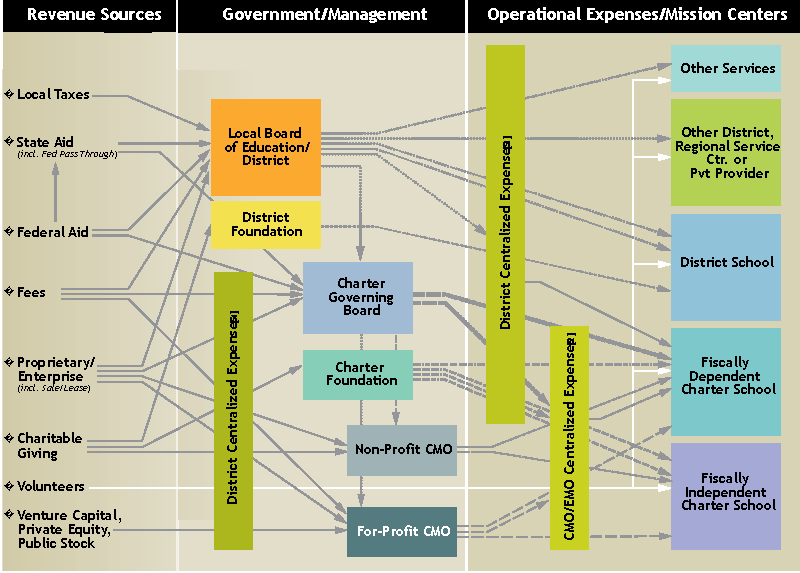
\includegraphics[width=\textwidth]{Operating_Resource_Flows}\\
  \footnotesize\raggedright\textcite[16]{Baker.Miron2015}.
\end{figure}
In this example, money flows from left to right, and there are no loops. Colors are used merely to distinguish the various blocks.

%%% Local Variables:
%%% mode: latex
%%% TeX-master: "Rocketship_Education-An_Exploratory_Public_Policy_Case_Study"
%%% TeX-command-extra-options: "-recorder"
%%% End:
